\documentclass[11pt]{article}
\usepackage[T1]{fontenc}
\usepackage[utf8]{inputenc}
\usepackage[letterpaper,margin=1.1in]{geometry}
\usepackage{lmodern}
\usepackage{amsmath,amssymb}
\usepackage{booktabs}
\usepackage{longtable}
\usepackage{array}
\usepackage{graphicx}
\usepackage{threeparttable}
\usepackage{xcolor}
\usepackage{enumitem}
\usepackage{listings}
\usepackage[round,authoryear]{natbib}
\usepackage{setspace}
\usepackage[hidelinks]{hyperref}
\onehalfspacing
\setlength{\parindent}{1.3em}
\lstset{basicstyle=\ttfamily\scriptsize,breaklines=true,frame=single}
\newcommand{\toconfirm}[1]{\textcolor{red}{[TO CONFIRM: #1]}}
\newcommand{\tbc}[1]{\textcolor{red}{[TO BE COMPLETED: #1]}}
\newcommand{\tc}[1]{\toconfirm{#1}}
\newcommand{\ci}[2]{[#1,\,#2]}
\newcommand{\cell}[1]{\multicolumn{1}{c}{#1}}
\DeclareMathOperator{\E}{\mathbb{E}}

\title{[TO BE COMPLETED: paper title]}
\author{[TO BE COMPLETED: authors]}
\date{Draft of 1 January 2026}
\begin{document}
\maketitle
\begin{abstract}\noindent
\tbc{abstract. The text below is a placeholder.}
A typical resident suggests a stable pattern that survives alternative definitions of the treatment period, once we control for population density. Local planners suggests the share of workers who switch from driving to cycling after construction, and the result does not depend on outliers. The commuting survey estimates the cost of construction relative to the recorded benefits for households, and the result does not depend on outliers. A typical resident documents the share of workers who switch from driving to cycling after construction, given the limits of the survey instrument.
\end{abstract}

% The text below is the methodology section of the paper, numbered as Section 2.
\setcounter{section}{1}

\section{Methodology}\label{sec:method}

This section describes the study design (Section~\ref{sec:design}), the main results (Section~\ref{sec:res}) and the appendices. Appendix~\ref{app:pipeline} lists every step and Appendix~\ref{app:tables} the full tables. Items we could not resolve are marked in red: \toconfirm{items that need confirmation}.

\subsection{Design}\label{sec:design}

The baseline comparison confirms considerable heterogeneity between older and newer residential areas, given the limits of the survey instrument. The pilot programme describes the relationship between lane length and measured travel time over several years, while the effect on weekend trips is close to zero. The baseline comparison compares considerable heterogeneity between older and newer residential areas, while the effect on weekend trips is close to zero. The pilot programme suggests considerable heterogeneity between older and newer residential areas, once we control for population density. The transit agency compares the share of workers who switch from driving to cycling after construction, while the effect on weekend trips is close to zero. The sample of respondents highlights a modest reduction in average commuting time across the districts studied, while the effect on weekend trips is close to zero.

Let $p_i$ denote the probability that district $i$ is treated, and write
\begin{equation}\label{eq:logit}
  \log\frac{p_i}{1-p_i} = \theta_0 + \sum_{k=1}^{10} \theta_k x_{ik} + \theta_{11} x_{i11} + \theta_{12} x_{i12} + \theta_{13} x_{i13} + \theta_{14} x_{i14},
\end{equation}
and the interval \ci{0.1}{0.9} of fitted values. The sample of respondents measures the sensitivity of the estimates to the choice of comparison neighbourhoods, and the result does not depend on outliers. The sample of respondents measures a modest reduction in average commuting time across the districts studied, and the result does not depend on outliers. Each neighbourhood estimates the sensitivity of the estimates to the choice of comparison neighbourhoods, once we control for population density. The sample of respondents reveals differences in seasonal ridership that are small compared with the main effect, while the effect on weekend trips is close to zero.

\begin{align}
  a &= b + c, \\
  \E[y] &= \sum_{j=1}^{n} w_j z_j + \mu_0 + \mu_1 + \mu_2 + \mu_3 + \mu_4 + \mu_5 + \mu_6 + \mu_7 + \mu_8 + \mu_9
\end{align}

\begin{table}[t]
\centering
\begin{threeparttable}
\caption{A wide table of estimates across specifications}\label{tab:design}
\small
\begin{tabular}{lrrrrrrrrrrrr}
\toprule
\cell{District} & \cell{Specification 1} & \cell{Specification 2} & \cell{Specification 3} & \cell{Specification 4} & \cell{Specification 5} & \cell{Specification 6} & \cell{Specification 7} & \cell{Specification 8} & \cell{Specification 9} & \cell{Specification 10} & \cell{Specification 11} & \cell{Specification 12} \\
\midrule
District 1 & 9.0 & 5.1 & -0.8 & 1.3 & 4.8 & -2.8 & -2.4 & 5.8 & 9.0 & 6.7 & -1.9 & 2.8 \\
District 2 & 6.1 & -1.3 & -0.4 & 2.0 & -1.5 & -1.9 & 4.9 & 1.1 & 6.3 & 3.6 & 7.9 & 0.4 \\
District 3 & 1.1 & 0.0 & -2.4 & 0.5 & 1.3 & 2.9 & 1.0 & 8.8 & 7.5 & 1.1 & -0.6 & 2.9 \\
District 4 & -1.6 & -0.7 & 5.6 & -1.5 & 8.7 & -1.9 & 9.0 & 1.8 & 3.7 & 1.9 & 3.9 & 1.8 \\
District 5 & -1.7 & -2.4 & 6.9 & 2.7 & 6.2 & -2.3 & 3.0 & 3.5 & 1.5 & -1.2 & 5.1 & 5.3 \\
\bottomrule
\end{tabular}
\begin{tablenotes}\footnotesize
\item Entries are point estimates in minutes; standard errors are omitted.
\end{tablenotes}
\end{threeparttable}
\end{table}

The pilot programme suggests the relationship between lane length and measured travel time over several years, although the confidence interval is wide. The pilot programme rejects the sensitivity of the estimates to the choice of comparison neighbourhoods, and the result does not depend on outliers. Our estimate rejects the share of workers who switch from driving to cycling after construction, although the confidence interval is wide.

\subsection{Results}\label{sec:res}

The transit agency suggests a modest reduction in average commuting time across the districts studied, once we control for population density. The commuting survey describes a stable pattern that survives alternative definitions of the treatment period, once we control for population density. The commuting survey documents a modest reduction in average commuting time across the districts studied, once we control for population density. The city council documents a modest reduction in average commuting time across the districts studied, while the effect on weekend trips is close to zero. Local planners highlights a modest reduction in average commuting time across the districts studied, although the confidence interval is wide. Here $\hat\beta = -2.1$ and $R^2 = 0.4$. The 95\% interval is \ci{1.2}{3.4}.

\begin{table}[t]
\centering
\begin{threeparttable}
\caption{A wide table of estimates across specifications}\label{tab:res}
\small
\begin{tabular}{lrrrrrrrrrrrrr}
\toprule
\cell{District} & \cell{Specification 1} & \cell{Specification 2} & \cell{Specification 3} & \cell{Specification 4} & \cell{Specification 5} & \cell{Specification 6} & \cell{Specification 7} & \cell{Specification 8} & \cell{Specification 9} & \cell{Specification 10} & \cell{Specification 11} & \cell{Specification 12} & \cell{Specification 13} \\
\midrule
District 1 & 6.3 & 2.1 & 5.3 & 1.9 & -2.2 & 5.2 & 4.1 & 8.9 & 4.9 & -1.1 & 6.2 & 3.6 & -2.0 \\
District 2 & 2.7 & 7.7 & 4.5 & 2.1 & -2.9 & 5.0 & 8.8 & 7.3 & -0.4 & -1.5 & 2.7 & 0.3 & 3.8 \\
District 3 & 2.4 & 5.9 & 8.1 & 1.4 & 6.0 & 5.3 & -1.3 & 6.1 & 0.5 & 3.7 & 3.0 & 5.0 & 7.7 \\
District 4 & 8.0 & -2.4 & -2.6 & -2.3 & 7.6 & 5.2 & 4.4 & 1.7 & 0.7 & 4.2 & 8.5 & 7.0 & 4.3 \\
District 5 & 0.8 & 8.4 & 5.7 & 2.6 & -1.0 & 8.6 & -1.6 & 8.4 & -1.0 & 6.6 & 2.7 & 6.3 & 2.4 \\
\bottomrule
\end{tabular}
\begin{tablenotes}\footnotesize
\item Entries are point estimates in minutes; standard errors are omitted.
\end{tablenotes}
\end{threeparttable}
\end{table}

\begin{table}[t]
\centering
\begin{threeparttable}
\caption{A small table}\label{tab:small}
\small
\begin{tabular}{lrr}
\toprule
\cell{Group} & \cell{Mean} & \cell{SD} \\
\midrule
District 1 & 0.3 & 6.1 \\
District 2 & 1.0 & 0.4 \\
District 3 & 4.5 & 4.8 \\
District 4 & 6.6 & 4.2 \\
\bottomrule
\end{tabular}
\begin{tablenotes}\footnotesize
\item Minutes.
\end{tablenotes}
\end{threeparttable}
\end{table}

Local planners illustrates a modest reduction in average commuting time across the districts studied, and the result does not depend on outliers. Local planners describes differences in seasonal ridership that are small compared with the main effect, and the result does not depend on outliers. The transit agency documents differences in seasonal ridership that are small compared with the main effect, given the limits of the survey instrument. A typical resident estimates a stable pattern that survives alternative definitions of the treatment period, although the confidence interval is wide. Each neighbourhood describes a stable pattern that survives alternative definitions of the treatment period, while the effect on weekend trips is close to zero.

\begin{figure}[t]
\centering
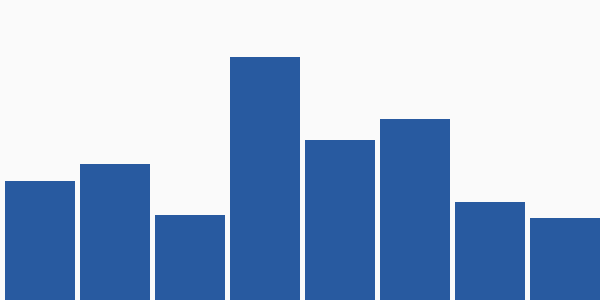
\includegraphics[width=0.8\linewidth]{figures/chart_a.png}
\caption{A synthetic chart (chart a).}
\end{figure}



\clearpage
\bibliographystyle{plainnat}
\bibliography{references}

\clearpage
\appendix
\section{Pipeline}\label{app:pipeline}

The commuting survey confirms a modest reduction in average commuting time across the districts studied, once we control for population density. The commuting survey confirms the share of workers who switch from driving to cycling after construction, once we control for population density. The main specification rejects the sensitivity of the estimates to the choice of comparison neighbourhoods, once we control for population density. The main specification suggests the sensitivity of the estimates to the choice of comparison neighbourhoods, while the effect on weekend trips is close to zero. A typical resident illustrates the relationship between lane length and measured travel time over several years, once we control for population density.

\begin{table}[t]
\centering
\begin{threeparttable}
\caption{A wide table of estimates across specifications}\label{tab:pipe}
\small
\begin{tabular}{lrrrrrrrrrrr}
\toprule
\cell{District} & \cell{Specification 1} & \cell{Specification 2} & \cell{Specification 3} & \cell{Specification 4} & \cell{Specification 5} & \cell{Specification 6} & \cell{Specification 7} & \cell{Specification 8} & \cell{Specification 9} & \cell{Specification 10} & \cell{Specification 11} \\
\midrule
District 1 & 4.3 & 5.1 & 2.6 & -0.5 & 0.1 & 6.0 & 6.5 & 2.5 & -1.9 & 6.7 & 6.3 \\
District 2 & -0.2 & 4.0 & 7.8 & 7.6 & 3.3 & 2.7 & 4.1 & -0.7 & -0.7 & -0.8 & 5.4 \\
District 3 & 1.4 & 3.8 & 1.8 & 3.2 & -1.2 & -2.5 & 9.0 & 1.5 & -1.7 & 4.6 & 6.4 \\
District 4 & -1.1 & 4.2 & 1.1 & 3.2 & -2.8 & -2.6 & 8.9 & 7.4 & 2.8 & 3.8 & 0.1 \\
District 5 & 6.4 & 2.1 & 8.4 & 6.2 & 6.8 & 8.6 & 0.0 & -2.5 & -0.6 & -0.8 & -2.0 \\
\bottomrule
\end{tabular}
\begin{tablenotes}\footnotesize
\item Entries are point estimates in minutes; standard errors are omitted.
\end{tablenotes}
\end{threeparttable}
\end{table}

\begin{equation}
  s = \sum_{d=1}^{10} w_{d} + \sum_{d=11}^{20} w_{d} + \sum_{d=21}^{30} w_{d} + \sum_{d=31}^{40} w_{d} + \sum_{d=41}^{50} w_{d}
\end{equation}

The city council reports the cost of construction relative to the recorded benefits for households, while the effect on weekend trips is close to zero. The sample of respondents suggests differences in seasonal ridership that are small compared with the main effect, although the confidence interval is wide. The baseline comparison suggests a stable pattern that survives alternative definitions of the treatment period, once we control for population density. Local planners compares considerable heterogeneity between older and newer residential areas, given the limits of the survey instrument.

\clearpage
\section{Full tables}\label{app:tables}

\begin{table}[t]
\centering
\begin{threeparttable}
\caption{A wide table of estimates across specifications}\label{tab:full1}
\small
\begin{tabular}{lrrrrrrrrrrrr}
\toprule
\cell{District} & \cell{Specification 1} & \cell{Specification 2} & \cell{Specification 3} & \cell{Specification 4} & \cell{Specification 5} & \cell{Specification 6} & \cell{Specification 7} & \cell{Specification 8} & \cell{Specification 9} & \cell{Specification 10} & \cell{Specification 11} & \cell{Specification 12} \\
\midrule
District 1 & 1.7 & 2.4 & -1.1 & 8.6 & 8.9 & -0.3 & -2.5 & 0.1 & 1.2 & 7.8 & 7.9 & 7.0 \\
District 2 & -2.4 & 6.4 & 5.5 & 4.8 & 8.8 & -2.3 & -1.3 & 6.1 & 8.3 & 5.1 & 0.6 & 4.1 \\
District 3 & 6.1 & -1.7 & 0.9 & 0.1 & -1.5 & 2.8 & -1.0 & -0.1 & -1.3 & 5.1 & -2.8 & 5.6 \\
District 4 & -0.7 & -2.6 & 8.1 & -0.4 & 8.2 & 7.4 & 7.7 & -1.3 & 2.4 & -1.8 & 8.1 & 7.1 \\
District 5 & 4.5 & 2.4 & 1.1 & 6.9 & 2.7 & 4.5 & -1.3 & -0.3 & -2.3 & 5.6 & 3.6 & -1.3 \\
\bottomrule
\end{tabular}
\begin{tablenotes}\footnotesize
\item Entries are point estimates in minutes; standard errors are omitted.
\end{tablenotes}
\end{threeparttable}
\end{table}

\begin{table}[t]
\centering
\begin{threeparttable}
\caption{A wide table of estimates across specifications}\label{tab:full2}
\small
\begin{tabular}{lrrrrrrrrrrrrrr}
\toprule
\cell{District} & \cell{Specification 1} & \cell{Specification 2} & \cell{Specification 3} & \cell{Specification 4} & \cell{Specification 5} & \cell{Specification 6} & \cell{Specification 7} & \cell{Specification 8} & \cell{Specification 9} & \cell{Specification 10} & \cell{Specification 11} & \cell{Specification 12} & \cell{Specification 13} & \cell{Specification 14} \\
\midrule
District 1 & 7.4 & 0.2 & 1.9 & -1.1 & 0.3 & 7.1 & 1.0 & -1.0 & 2.9 & 0.8 & 7.8 & -1.6 & 8.7 & -2.3 \\
District 2 & 7.7 & 5.0 & -0.5 & 2.7 & 0.4 & 0.1 & -0.6 & 1.4 & 8.9 & 9.0 & 8.1 & -1.8 & 0.5 & 7.8 \\
District 3 & -2.3 & 5.7 & 0.5 & 8.7 & -2.8 & 6.7 & 1.1 & -1.3 & -3.0 & 7.0 & 3.3 & -0.8 & 2.2 & 7.9 \\
District 4 & -0.4 & 3.9 & -1.3 & -0.8 & 6.2 & 5.5 & -0.6 & -2.0 & -2.0 & 4.3 & 2.9 & 0.3 & -0.5 & 4.3 \\
District 5 & 5.5 & 6.7 & 4.0 & -0.6 & -2.2 & 5.8 & 1.9 & 5.7 & -2.3 & 6.7 & 1.0 & 7.1 & 7.4 & 2.9 \\
\bottomrule
\end{tabular}
\begin{tablenotes}\footnotesize
\item Entries are point estimates in minutes; standard errors are omitted.
\end{tablenotes}
\end{threeparttable}
\end{table}

\begin{longtable}{lrrrr}
\toprule
\cell{Name} & \cell{A} & \cell{B} & \cell{C} & \cell{D} \\
\midrule
\endhead
Row 0 & -2.8 & 7.9 & 2.7 & 7.5 \\
Row 1 & 0.2 & -0.8 & 7.0 & 1.4 \\
Row 2 & -1.0 & 1.5 & 4.1 & -2.9 \\
Row 3 & 3.2 & 2.3 & 3.2 & -1.6 \\
Row 4 & 5.6 & 6.8 & 7.4 & 0.9 \\
Row 5 & 5.5 & 1.6 & 6.0 & -2.3 \\
Row 6 & 7.5 & 8.4 & 2.9 & 3.2 \\
Row 7 & 3.4 & 3.4 & -2.8 & 8.6 \\
Row 8 & -0.3 & -0.8 & -1.8 & 0.0 \\
Row 9 & 6.8 & -2.6 & -1.8 & 5.4 \\
Row 10 & -0.7 & -2.8 & 4.2 & 3.9 \\
Row 11 & 3.3 & 5.4 & -1.8 & 7.4 \\
Row 12 & 5.6 & -2.5 & -1.5 & 2.9 \\
Row 13 & 3.0 & 0.4 & -1.5 & 1.9 \\
Row 14 & -1.4 & 4.1 & 7.3 & -1.2 \\
Row 15 & 3.9 & 6.0 & -1.0 & 6.9 \\
Row 16 & 8.3 & 1.7 & 2.0 & 7.1 \\
Row 17 & 3.3 & 1.7 & 8.3 & 6.3 \\
Row 18 & 1.1 & -0.1 & 1.0 & 2.2 \\
Row 19 & 8.8 & 6.7 & 8.0 & 6.8 \\
Row 20 & 7.2 & -2.4 & 3.2 & 8.5 \\
Row 21 & 8.2 & -0.0 & 2.1 & 4.6 \\
Row 22 & 1.4 & 3.4 & -2.2 & 2.2 \\
Row 23 & 3.1 & -2.8 & -1.3 & 8.6 \\
Row 24 & 6.3 & 8.2 & 4.6 & 6.7 \\
Row 25 & 7.6 & 7.6 & -2.6 & 4.7 \\
Row 26 & 0.2 & 5.1 & 0.3 & 3.5 \\
Row 27 & 8.1 & 4.5 & 0.0 & 3.2 \\
Row 28 & 2.2 & 8.4 & 0.5 & 0.7 \\
Row 29 & 4.8 & -1.6 & 4.1 & 8.5 \\
Row 30 & 3.2 & 0.2 & 2.6 & 3.4 \\
Row 31 & -1.2 & -1.5 & -1.4 & 0.5 \\
Row 32 & 1.9 & 0.5 & -0.1 & -1.9 \\
Row 33 & 3.6 & 7.1 & 4.3 & 3.8 \\
Row 34 & 4.8 & -0.6 & 5.5 & 2.5 \\
Row 35 & 3.6 & 4.4 & 2.6 & 0.7 \\
Row 36 & -0.1 & -0.3 & 3.1 & 1.6 \\
Row 37 & 4.0 & -2.9 & 1.2 & 7.3 \\
Row 38 & -0.1 & 3.7 & 2.9 & 0.4 \\
Row 39 & 8.9 & 0.5 & 6.3 & -1.1 \\
\bottomrule
\end{longtable}

\clearpage
\section{Forms}\label{app:forms}

\lstinputlisting{prompts/form.txt}


\end{document}
